\comEC{Ajuster les temps au passé toujours}

% C'est important d'étudier les take-off au trampoline
The addition of flight time to trampoline score in 2010 \cite{Committee2010} has changed coaches' perception of ideal propulsion technique.
Achieving high somersault velocity while maintaining important jumping height has become more important than ever.
The complexity of this task lies in generating linear and angular momenta at the same time.
The first one is maximal when the force generated by the trampoline force is aligned with the center of mass (CoM) of the athlete (Left image in Fig~\ref{fig:Linear_vs_angular_mom}), while the second is maximal perpendicularly, i.e. when the force is orthogonal to the vector feet-CoM, maximizing the moment arm (center image in Fig~\ref{fig:Linear_vs_angular_mom}).
Therefore a compromise is needed at each instant during the propulsion phase.
% Even though coaches are able to recognize visually the quality of a take-off, it stays challenging to formulate feedback for athletes because kinematic errors might originate from different sources.
% The athlete might not perform the desired motor patern due to strength limitations, active flexibility limitations, lack of coordination  or bad timing.
Without a deeper insight into the biomechanics of the take-off, it is challenging to determine the optimal timeline of actions that should be executed by the athlete during the contact phase.

\begin{figure}[h!]
\centering
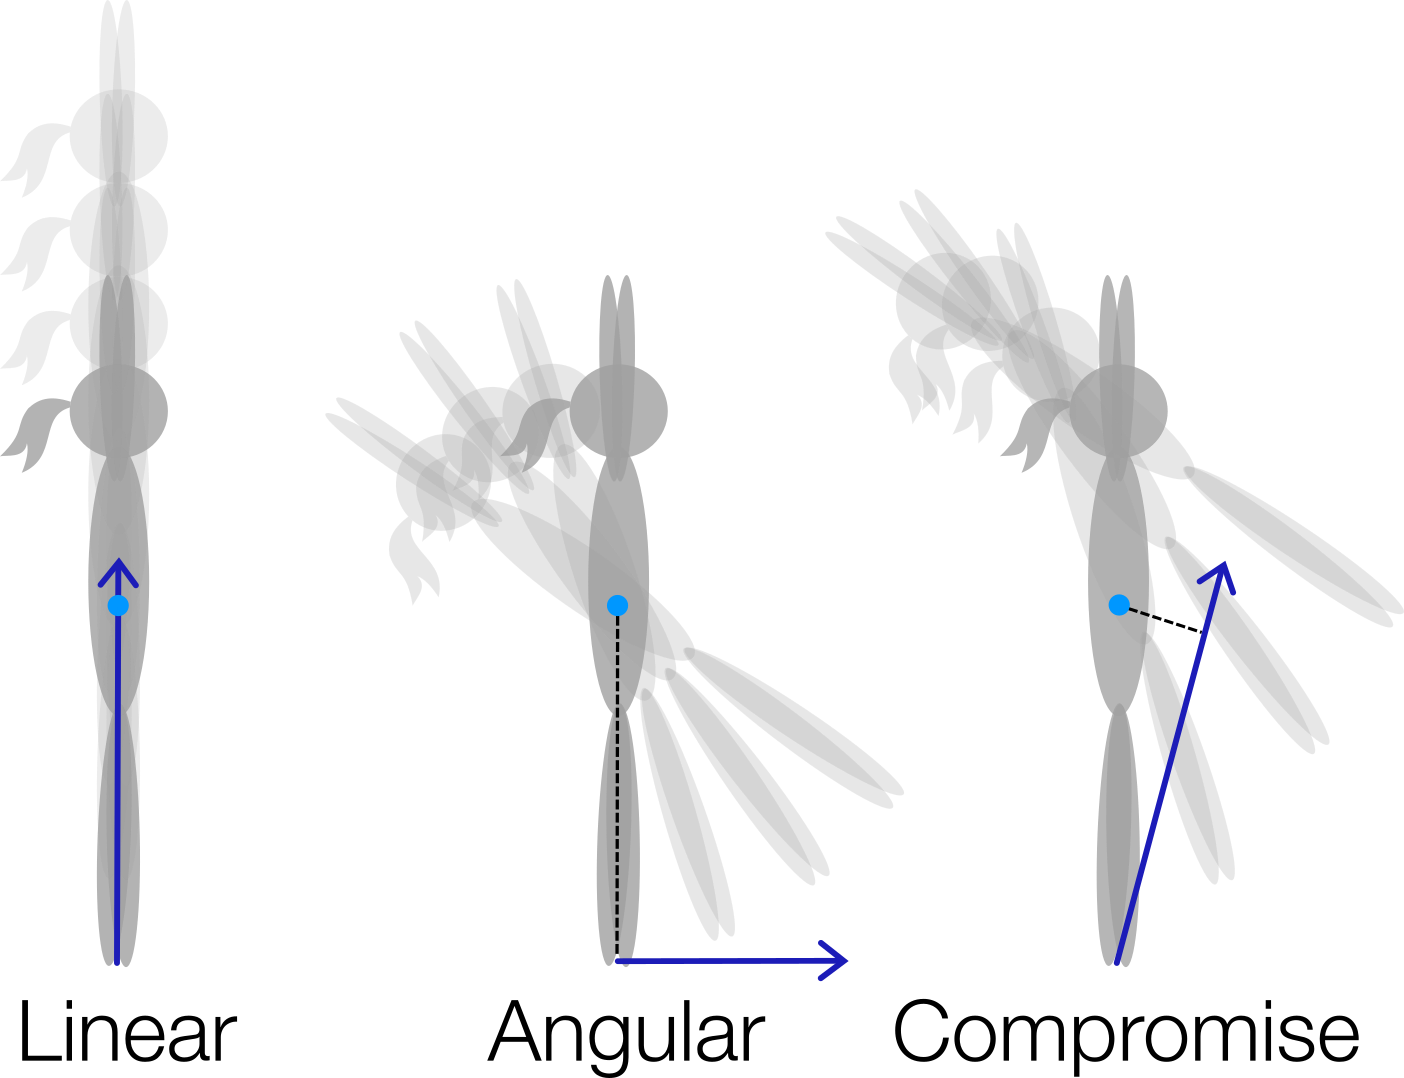
\includegraphics[width=0.8\linewidth]{figures/Linear_vs_angular_mom.png}
\caption{Illustration of the effect of the orientation of the force on the angular and linear momenta. 
The linear momentum is maximal in the left image. 
The angular momentum is maximal in center image. 
Both linear and angular momenta are generated in the right image.}
\label{fig:Linear_vs_angular_mom}
\end{figure}

% Le meilleur model de toile c'est celui de Jacques2008
The first step to analyze athlete-trampoline interaction is to investigate the force applied by the trampoline on the athlete.
However, measuring this force is challenging due to the movement of the contact point.
In order to quantify it, some studies used force transducers under the trampoline supports \cite{jacques2008determining, ando1987biomechanical, hennig1988loads}, insoles \cite{glitsch1992pressure} or tri-axial accelerometers placed on the athlete \cite{eager2012characterisation}.
Other studies used a combination of modeling and video recording to estimate the force generated by the trampoline \cite{vaughan1980kinetic, blajer2001modeling, zuo2016finite, burke2015mechanics}.
These indirect techniques leverage the relationship between the trampoline deformation and the force generation.
These methods have the advantage to simply model the trampoline's force-displacement relationship with polynomial expressions.
However, in order to calibrate the parameters of these models, drop and load tests are usually needed.
These tests get more dangerous as the trampoline deformation increases, especially horizontally, therefore it becomes risky to match the level of bed depression achieved by athletes (up to 1 meter).
\comFB{ Bizarre de parler d'une depression horizontale. -> pour ca que je dis deformation a la place}
In these circumstances, force-displacement relationships could not be fully confirmed with experimental data. 
It could only be hypothesized that the tendency would be preserved throughout larger bed deformations.
Finally, one study used more complex modeling enabling to estimate the force from static measurements on springs and bed separately \cite{jacques2008determining}.
This technique has the advantage to reliably estimate vertical and horizontal forces at the same time while providing a safer data collection.


% C'est important de tenir en compte la force vertical et horizontale dans analyses et modelisation
Until now, trampoline forces were studied with an emphasis on the vertical component.
However, the trampoline bed and spring system has the ability to deform both vertically and horizontally giving rise to a three dimensional force (Fig.~\ref{fig:Visu_force_ori}).
For non-twisting somersault, the component of the force in the frontal plane must be null to avoid lateral displacements during the flight phase.
The same logic does not apply for the sagittal plane because the athlete's motion \comFB{which part of the motion ?}
generating somersault happen in this plane.
Indeed, sagittal plane motions enlarging the contribution to angular momentum include three strategies: \textit{i)} shift the CoM, \textit{ii)} change the orientation of the force at the application point or \textit{iii)} move the application point.
Forward somersaulting take-off strategies were investigated to analyze CoM and feet trajectories to assess the biomechanical strategies leading to generation of angular and linear momentum \cite{lephartatiner}.
\comFB{Pourquoi est-ce qu'on passe aux forward somersault ? -> pcq il a juste fait ca et je trouvais important de le mentionner ?}
Strategies involving solely vertical force on the trampoline were qualified as not viable due to the loss of height and horizontal displacement they imply \cite{lephartatiner}.
\comFB{Cela est sense justifier le modele 3d du trampo ? -> oui /  Tu veux dire que la seule strategie viable est ii) ? -> Non}
Therefore, it seems necessary to analyze both horizontal and vertical bed work.

\comEC{Fig.~\ref{fig:Visu_force_ori} peut-être plus a mettre en annexe selon si on vise un journal appliqué ou pas}
\begin{figure}[h!]
\centering
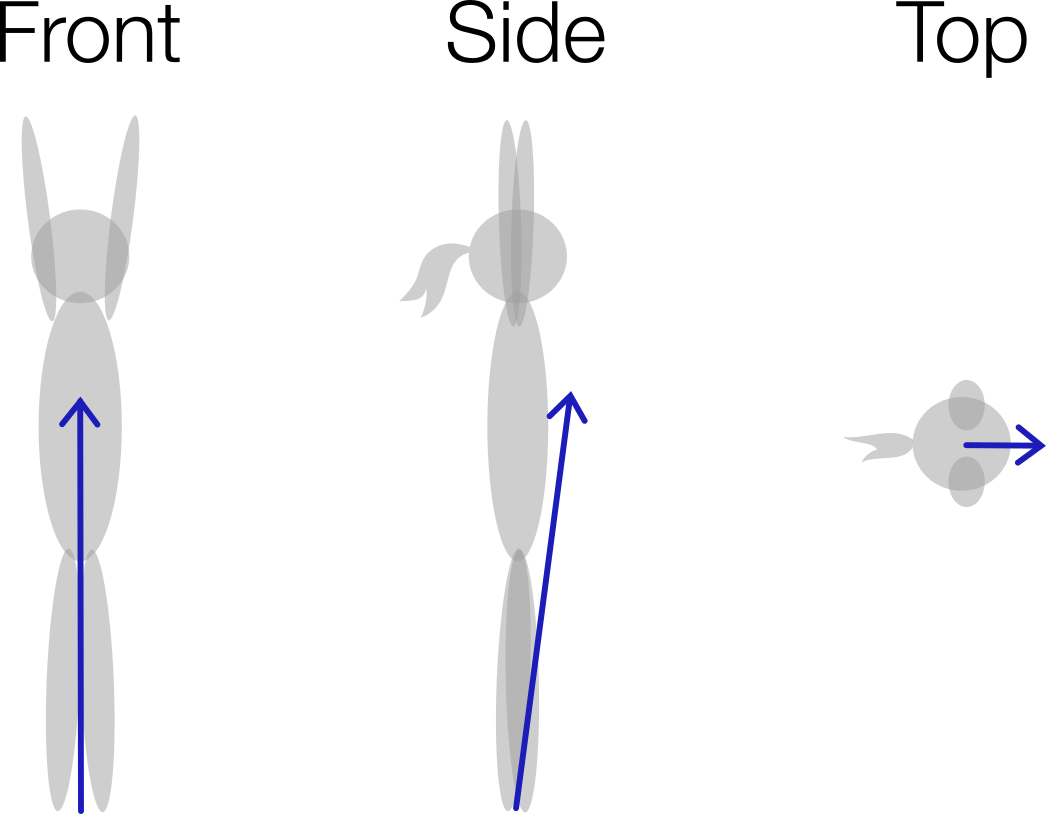
\includegraphics[width=0.8\linewidth]{figures/Visu_force_ori.png}
\caption{Illustration of the orientation of the force at one instant during the take-off of a non-twisting backward somersault from front (left image), side (center image) and top (right image) view.}
\label{fig:Visu_force_ori}
\end{figure}

% Le controle optimal est un bon outil pour étudier les take-offs
Optimal control is a relevant tool to study sport techniques because it helps (in)validate the techniques currently used \cite{charbonneau2020optimal}.
Indeed, it allows to identify biomechanical strategies and provide advises to the sport community accordingly.
Jumping motion on compliant surfaces have rarely been studied by means of numerical optimization \cite{cheng2008role, burke2015mechanics}.
When they were, only one type of acrobatic skill was considered, i.e. backward or forward somersaults.
However, trampolining is composed of both types of skills, typically combined in alternation to compose the required 10-skills routine. 
Therefore, studying the transition between skills is more relevant than single skills to the sport community.
Moreover, the optimization must include the contact phase and the aerial phase of the studied skills, as both are interdependent, e.g., a bad posture during take off might impact negatively the beginning of the flight phase. 


% A la fois les modeles de toile et d'athlete doivent être assez complexes pour représenter la réalité 
To draw biomechanical conclusions from strategies found by optimization, the model must be validated with experimental data, like it was the case for the athlete model used in \cite{burke2015mechanics}.
% It was torque actuated, however torque values were non linearly bounded to physiological values.
The biggest challenge associated with this model was it's lack of degrees of freedom (DoF); it was mentionned that the addition of one shoulder and one thoracic DoF would be beneficial.
Similarly, the trampoline model used in \cite{jacques2008determining} showed a great level of accordance with experimental data.
\comEC{Ca dit que c'est le meilleur qui existe mais qu'il reste du travail a faire :(}
However, both trampoline and athlete models were never used in conjunction in an OCP with this level of modelling complexity.


The first aim of this study was to find bed work techniques \comFB{bed work techniques ? -> pas une bonne expression ?} generating somersaults at maximal height in trampoline. 
A secondary objective was to identify the limiting factors by providing a biomechanical analysis of the underlying strategies.
\comFB{pas très clair}
% We hypothesized that for the same number of somersault completed, the height of the avatar taking advantage of 2D force would be grater than for the avatar propelled by 1D force only. 


\comEC{Étude de sensibilité littérature? (force, flex épaules, morphologie)}
% The studies addressing trampoline jumping optimization offered a vertical representation of the contact force (referred to as \textit{1D force}), however the force applied on the athlete's feet has three components. 
% 2D modeling of the trampoline contact force, referred to as \textit{2D force}, would allow to fully use the trampoline deformation to generate somersault of maximal height.
\comFB{À la fin de ton intro, on ne sait pas vraiment ce que tu vas faire. On ne sait pas si tu vas retravailler un modèle de trampo, etc.}
